\documentclass[aspectratio=43,english]{beamer} %If you want to create Polish presentation, replace 'english' with 'polish' and uncomment 3-th line, i.e., '\usepackage{polski}'
\usepackage[utf8]{inputenc}
\usepackage{polski} %Uncomment for Polish language
\usepackage{babel}
\usepackage{listings} %We want to put listings

\mode<beamer>{ 	%in 'beamer' mode
	\hypersetup{pdfpagemode=FullScreen}		%Enable Full screen mode
	\usetheme{JuanLesPins} 		%Show part title in right footer
	%\usetheme[dark]{AGH}                 		%Use dark background
	%\usetheme[dark,parttitle=leftfooter]{AGH}  	%Use dark background and show part title in left footer
}
\mode<handout>{	%in 'handout' mode
	\hypersetup{pdfpagemode=None}		
	\usepackage{pgfpages}
  	\pgfpagesuselayout{4 on 1}[a4paper,border shrink=5mm,landscape]	%show 4 slides on 1 page
  	\usetheme{boxes}
  	\addheadbox{structure}{\quad\insertpart\hfill\insertsection\hfill\insertsubsection\qquad} 	%content of header
 	\addfootbox{structure}{\quad\insertauthor\hfill\insertframenumber\hfill\insertsubtitle\qquad} 	%content of footer
}

\AtBeginPart{ %At begin part: display its name
	\frame{\partpage}
} 


%%%%%%%%%%% Configuration of the listings package %%%%%%%%%%%%%%%%%%%%%%%%%%
% Source: https://en.wikibooks.org/wiki/LaTeX/Source_Code_Listings#Using_the_listings_package
%%%%%%%%%%%%%%%%%%%%%%%%%%%%%%%%%%%%%%%%%%%%%%%%%%%%%%%%%%%%%%%%%%%%%%%%%%%%
\lstset{ %
  backgroundcolor=\color{white},   % choose the background color
  basicstyle=\footnotesize,        % the size of the fonts that are used for the code
  breakatwhitespace=false,         % sets if automatic breaks should only happen at whitespace
  breaklines=true,                 % sets automatic line breaking
  captionpos=b,                    % sets the caption-position to bottom
  commentstyle=\color{green},      % comment style
  deletekeywords={...},            % if you want to delete keywords from the given language
  escapeinside={\%*}{*)},          % if you want to add LaTeX within your code
  extendedchars=true,              % lets you use non-ASCII characters; for 8-bits encodings only, does not work with UTF-8
  frame=single,	                   % adds a frame around the code
  keepspaces=true,                 % keeps spaces in text, useful for keeping indentation of code (possibly needs columns=flexible)
  keywordstyle=\color{blue},       % keyword style
  morekeywords={*,...},            % if you want to add more keywords to the set
  numbers=left,                    % where to put the line-numbers; possible values are (none, left, right)
  numbersep=5pt,                   % how far the line-numbers are from the code
  numberstyle=\tiny\color{gray},   % the style that is used for the line-numbers
  rulecolor=\color{black},         % if not set, the frame-color may be changed on line-breaks within not-black text (e.g. comments (green here))
  showspaces=false,                % show spaces everywhere adding particular underscores; it overrides 'showstringspaces'
  showstringspaces=false,          % underline spaces within strings only
  showtabs=false,                  % show tabs within strings adding particular underscores
  stepnumber=2,                    % the step between two line-numbers. If it's 1, each line will be numbered
  stringstyle=\color{cyan},        % string literal style
  tabsize=2,	                   % sets default tabsize to 2 spaces
  title=\lstname,                  % show the filename of files included with \lstinputlisting; also try caption instead of title
                                   % needed if you want to use UTF-8 Polish chars
  literate={?}{{\k{a}}}1
           {?}{{\k{A}}}1
           {?}{{\k{e}}}1
           {?}{{\k{E}}}1
           {�}{{\'o}}1
           {�}{{\'O}}1
           {?}{{\'s}}1
           {?}{{\'S}}1
           {?}{{\l{}}}1
           {?}{{\L{}}}1
           {?}{{\.z}}1
           {?}{{\.Z}}1
           {?}{{\'z}}1
           {?}{{\'Z}}1
           {?}{{\'c}}1
           {?}{{\'C}}1
           {?}{{\'n}}1
           {?}{{\'N}}1
}
%%%%%%%%%%%%%%%%%


\title{Metody Obliczeniowe w Nauce i Technice}
\author{Marian Bubak, PhD}
\date{}
\institute[AGH]{
	Institute of Computer Science\\ul. Kawiory 21\\30-055 Krakow\\
	Poland\\
	\url{http://www.icsr.agh.edu.pl/~mownit/}
}



%%%%%%%%%%%%%%%%%%%%%%
\usepackage{amsmath}
\usepackage{mathtools}
\usepackage{setspace}
\usepackage{scrextend}
\usepackage{listings}
%%%%%%%%%%%%%%%%%%%%%%

\subtitle{14. Liczby losowe (random numbers)}
\setcontributors{Dawid Prokopek\\Paweł Matejko\\Kamil Doległo}

	
\begin{document}
	\maketitle
	%%%%%%%%%%%%%%%%
	\begin{frame}{Plan wykładu}
		\tableofcontents
	\end{frame}
	%%%%%%%%%%%%%%%%
	\section{Wstęp}
	\begin{frame}{Wstęp}
    
    \textit{Komputer urządzenie precyzyjne, deterministyczne czy może służyć do produkowania liczb losowych !? }
    \newline

	\textbf{Historyczne rozróżnienie:}

	\textbf{random (losowe)}- uzyskiwane z procesów istotnie losowych (generatory fizyczne):
	
	- detektor Geigera-Müllera,

	- szum lamp elektronowych,

	- ruletka...

	\textbf{quasirandom (pseudolosowe)} - sekwencje generowane przez komputery (generatory programowe).
    
    $\newline$

	UWAGA: w symulacjach komputerowych potrzebujemy odtwarzalności, błędem jest rezygnacja z niej 
	\end{frame}
	%%%%%%%%%%%%%%%%
	\section{Liczby losowe o rozkładzie równomiernym (uniform deviate)}
\begin{frame}{Liczby losowe o rozkładzie równomiernym (uniform deviate)}


	Podstawowy typ generatora liczb losowych:
	\begin{center}
	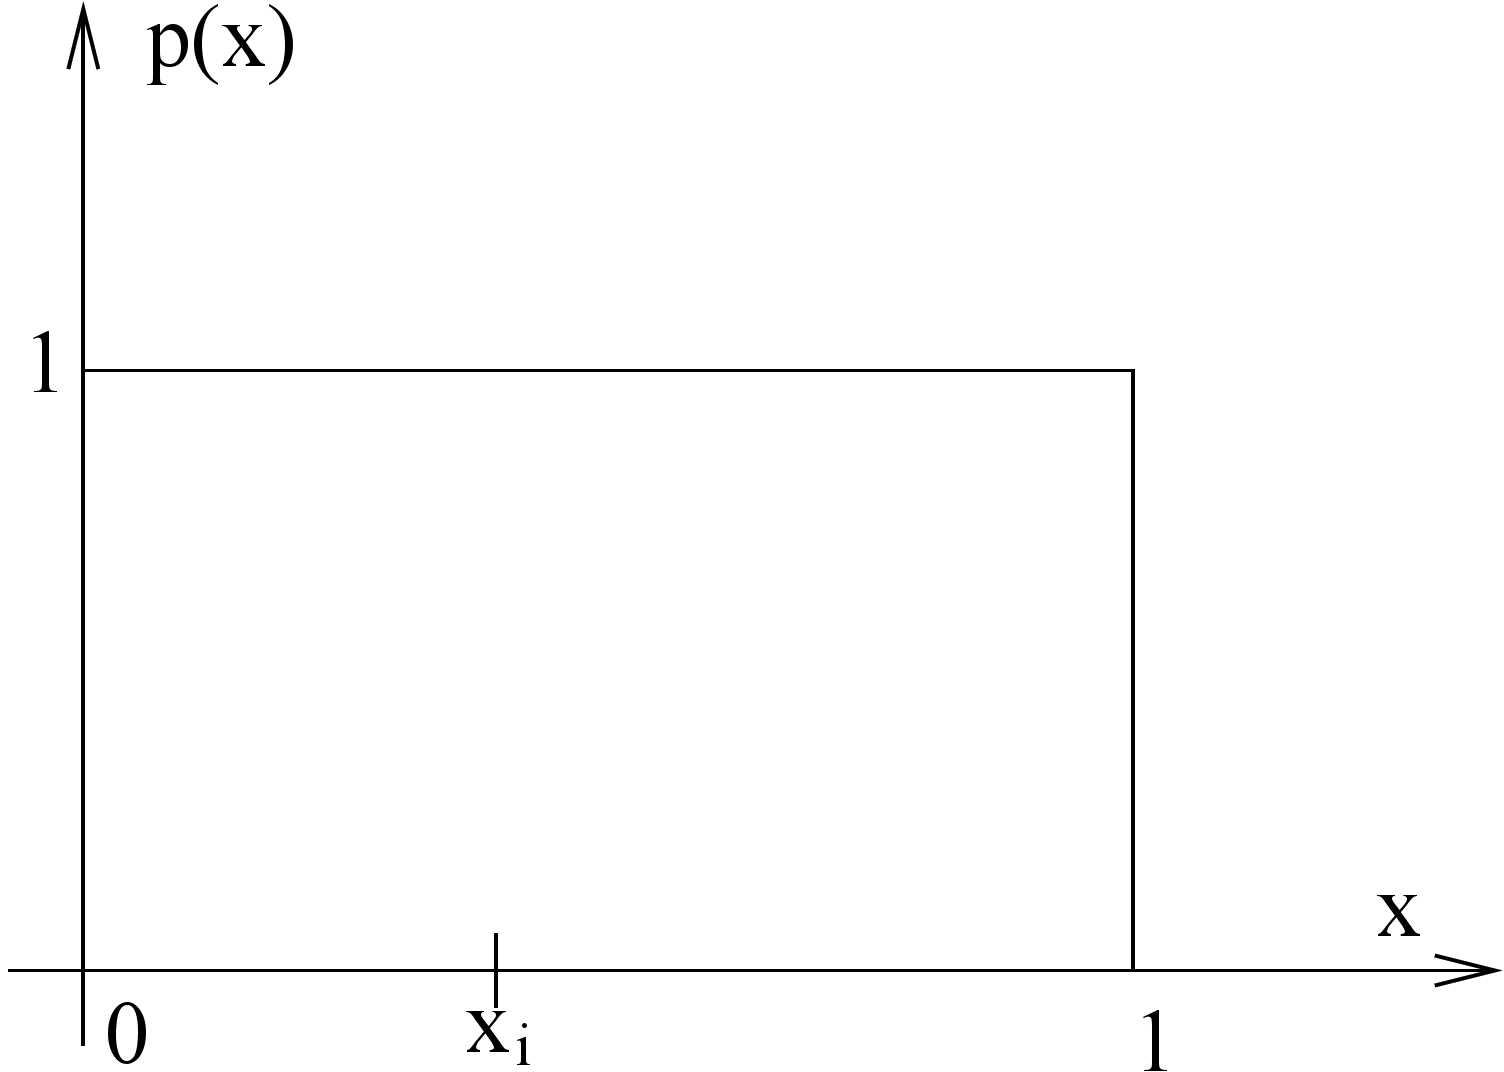
\includegraphics[scale=0.15]{img/14/14_2_img}
	\end{center}
    \end{frame}

    \begin{frame}
    \begin{exampleblock}{}
	$\{x_{i}\}-$ ciąg liczb z przedziału $(0,1)$ --równomierny na $(0,1)$, gdy:
	$$
	\forall(a,\ b)\ :\ 0\leq a\leq b\leq 1\ \lim_{N\rightarrow\infty}\frac{1}{N}\sum_{i/1}^{N}\eta_{a,b}		(x_{i})=b-a
	$$
	gdzie: $\eta_{a,b}=\left\{\begin{array}{l}
	1,\ a<x<b\\
	0,\ \mathrm{p}\mathrm{o}\mathrm{z}\mathrm{o}\mathrm{s}\mathrm{t}\mathrm{a}\mathrm{l}\mathrm{e}.
	\end{array}\right.$
	\end{exampleblock}
	W większości bibliotek programów procedura \textit{ranf}.

            \[
            	x = ranf(iseed)
            \]

	- pod $x$ podstaw następną liczbę losową \\
    - aktualizuj \textit{iseed}

	\textbf{iseed} --dowolna, zadawana przy pierwszym wywołaniu; \\
	- ta sama początkowa wartość $\Rightarrow$ ta sama sekwencja liczb pseudolosowych.
	\end{frame}

	%%%%%%%%%%%%%%%%
	\section{Generatory liczb równomiernych}
	\begin{frame}{Generatory liczb równomiernych}


	\textbf{14.3.1 Ogólne}
	\[
	x_{n+1}=f(\underbrace{x_{n},x_{n-1},\ldots,x_{n-k+1}}_{k \:stalych\: poczatkowych}) (mod\ \ M)
	\]
	Zal:
	$$
	D(f)=Z_{M}=\{0,\ 1,\ .\ .\ .\ ,\ M-1\}
	$$
	$$
	D^{-1}(f)=Z_{M}
	$$
	Takie generatory są {\it okresowymi}:
	\begin{center}
	$\exists N, K:\forall n\geq N x_{n}=x_{n}+jk$ , $j=1$, 2, . . .
	\end{center}
	$r$ -najmniejsza $N$:
    \begin{center}
	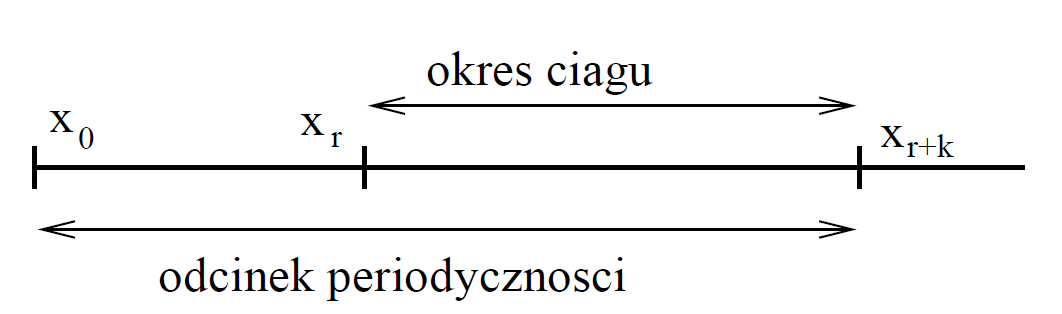
\includegraphics[width=70mm,height=20mm]{img/14/14_3_1_img}
	\end{center}
	\end{frame}

    \begin{frame}{Generatory liczb równomiernych}

	\textbf{14.3.2 Generator Fibonacciego}
	\begin{center}
 	$$x_{n+1} = (x_{n} + x_{n-1})(mod M)$$
	\end{center}
	- okres $\leq M^{2},$

	- prosty,

	- wada: korelacje w ciqgach generowanych liczb.
    \newline
	\end{frame}
    \begin{frame}
	\textbf{14.3.3 Generatory liniowe kongruentne}

	Większość generatorów to generatory {\it liniowe kongruentne}:\\ (1943, D.H. Lehmer)
	\begin{center}
 	$$I_{j+1} = (aI_{j}+c) mod\ m$$
	\end{center}
	gdzie:

    \[
    {\begin{rcases*}
	a - multiplier\\
	c - increment\\
	m - modulus
    \end{rcases*} liczby\ \ całkowite \ \ \in [0,m]}
    \]
	\end{frame}
    \begin{frame}
	Liczby zmiennoprzecinkowe: $\displaystyle \frac{I_{j+1}}{m}\in[0$, 1)
    \newline

	sekwencja: $I_{1}, I_{2}$, {\it I}3, . . . ; $0\leq I_{i}\leq m-1$
    \newline \newline
    okres $\leq m$ ; zalezy od wyboru $a, c \left\{\begin{array}{l}
	c\neq 0\ \rightarrow\ mieszane,\\
	c=0\ \rightarrow multiplikatywne.
	\end{array}\right.$

	Zaleta:

	a) {\it szybkość generacji}
	\newline

	Wady:

	a) {\it korelacje sekwencji}

	- $k$ -liczb losowych $\rightarrow$punkt w przestrzeni $k-D,$

	- punkty nie zapełniają r\'{o}wnomiernie przestrzeni lecz ukladają się na $(k-1)-D$ 				hiperplaszczyznach. Ilość plaszczyzn $\neq m^{\frac{1}{k}}, np. \ \ k=3, m=2^{32}\rightarrow 1600$ 		plaszczyzn

    \end{frame}
    \begin{frame}
	Kiedyś IBM wsławił się zdaniem ``{\it gwarantuje tylko losowośc każdej liczby indywidualnie }''
    \newline
    \newline
	b) {\it niższe bity są} ``{\it mniej losowe}'' niż {\it wyższe}:

    - nie wykorzystywać liczb losowych w {\it kawałkach},

	- np.do generowania liczb losowych $\in[1, 10 ]$

	używać:

	$J=1+INT(10.0*$RANF (iseed) $)$

	a nie:

	$J=1+MOD(INT(100000.0*RANF($iseed)$),\ 10)$
    \end{frame}

	%%%%%%%%%%%%%%%%
	\section{Zasady doboru stałych generatora liniowego kongruentnego}
	\begin{frame}{Zasady doboru stałych generatora liniowego kongruentnego}

 	 $I_{0}$: \\
 	 - nie ma większego znaczenia
	\newline \newline
	$a$: \\
	- $a(mod 8)=5$ \\
	- $\frac{m}{100}<a<m-\sqrt{m}$ \\
	- brak powtarzającego się wzorca w zapisie w systemie dwójkowym
	\newline \newline
	$c$: \\
	- nieparzyste \\
 	- $spełniające \frac{c}{m}\approx\frac{1}{2}-\frac{\sqrt{3}}{6}$
	\newline \newline
	$m$: \\
	$m=2^{t}$ , \quad t-liczba bitów przeznaczonych na 1 liczbę calkowitą


	\end{frame}

	%%%%%%%%%%%%%%%%
	\section{Zmniejszenie korelacji w sekwencji liczb losowych}
	\begin{frame}{Zmniejszenie korelacji w sekwencji liczb losowych}
	- procedura ''{\it losowego tasowania}'' (random shuffling procedure) {\it Bays-Durham 	$\Rightarrow Knuth$: ``The Art of Computer 	Programing'' vol. II.} 
	\newline \newline
	Uogólnienie:

	- kilka generatorów

	- jeden z nich wybiera ``dostarczyciela'' liczb

	\textbf{RANF} - generator systemowy,

	\textbf{RANO} - generator ulepszony

	\textbf{A} - tablica pomocnicza ( MX=97- l. pierwsza)

	\end{frame}
    
	\begin{frame}{Zmniejszenie korelacji w sekwencji liczb losowych}
		\centering 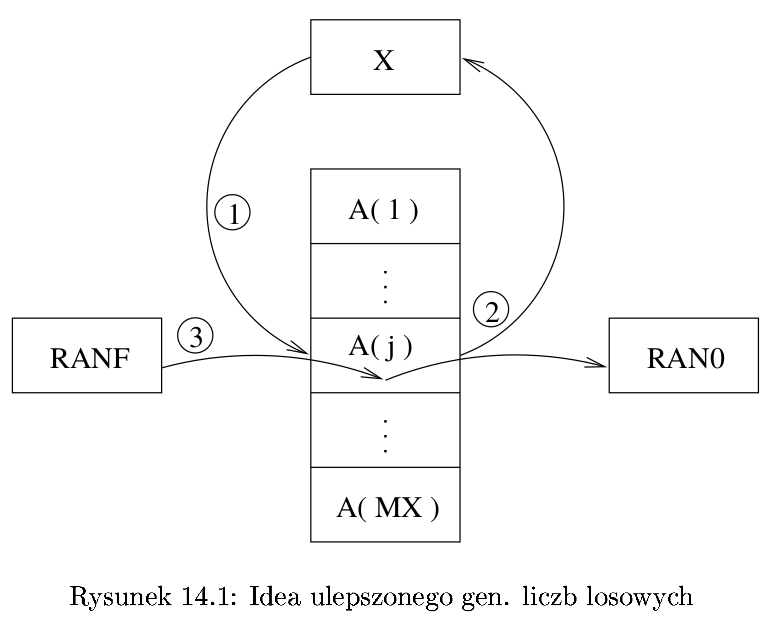
\includegraphics[width=.8\linewidth]{img/14/14_5_1_img.png}
	\end{frame}

	\begin{frame}{Zmniejszenie korelacji w sekwencji liczb losowych}
		\begin{enumerate}
			\setcounter{enumi}{-1}
			\item wypełnienie tablicy $A$ i zmiennej $x$ liczbami losowymi
			\item $x$ $\rightarrow$ $j$
			\item $A(j)$ $\rightarrow$ $l$. losowa $\rightarrow$ $x_{i}$ wyjście procedury
			\item z generatora systemowego $\rightarrow$ liczba losowa do $A(j)$
		\end{enumerate}
	\end{frame}

	\subsection{Ulepszony generator liczb losowych}
	\lstnewenvironment{code}{}{}
	
	\begin{code}
	function ran0(idum)
	parametr (MX = 97)
	real A(MX)
	data iff /0/
	
	                                     inicjacja
	if((idum.lt.0).or.(iff.eq.0)) then     -przy 1-szym
	    iff = 1                             wywolaniu
	    iseed = abs(idum)                  -gdy idum < 0
	    idum = 1
	    do 11 j = 1, MX
	        idum = ranf(iseed)             -przebiegi
	    continue                            jalowe gen.
	    do 12 j = 1, MX                     systemowego
	        A(j) = ranf(iseed)
	    x = ranf(iseed)
	endif
	
	\end{code}

	\begin{code}
	                                    przebieg roboczy
	j = 1 + int(MX * x)    - indeks
	if((j.gt.MX).or.(j.lt.1)) error()
	x = A(j)                               -z indeksu
	ran0 = x      - liczba losowa
	A(j) = ranj(iseed)                     -uzupelnienie
	return       tablicy
	end
	\end{code}

	%%%%%%%%%%%%%%%%
	\section{Zmienne losowe o zadanym rozkładzie}
\subsection{Metoda transformacji}
\begin{frame}{Zmienne losowe o zadanym rozkładzie\linebreak Metoda transformacji}
	\begin{block}{Podstawowe generatory - o rozkładzie równomiernym (uniform deviate):}
		\[
			P\left\{x < X < x + dx\right\} = p(x)dx = \begin{cases}
				dx,\hspace{0.5cm} 0 < x < 1\\
				0,\hspace{0.65cm} $ gdzie indziej$
			\end{cases}
		\]
		\[
			\fbox{$p(x) = 1$}
		\]
	\end{block}
\end{frame}
%%%%%%%%%%%%%%%
\begin{frame}{Metoda transformacji}
	\begin{block}{Generatory zmiennej losowej $y(x)$ o \textit{zadanym rozkładzie}
	$p(y)$:}
	\[
		\lvert p(y)dy \rvert \hspace{0.1cm} = \hspace{0.1cm} \lvert p(x)dx \rvert \hspace{6.8cm}
	\]
	\[
		\phantom{x} \hspace{0.2cm} p(y) \hspace{0.1cm} = \hspace{0.1cm} p(x) \left| \frac{dx}{dy} \right| \Rightarrow p(y) = \frac{dx}{dy}, \hspace{0.1cm} x = F(y) = \int_{0}^{y} p(y)dy
	\]
	\[
		\fbox{$y(x) = F^{-1}(x)$} \text{ ,} \hspace{1cm} F(y) - \text{dystrybuanta rozkładu p(y)}
	\]
	\end{block}
	\vspace{1cm}
	
	\flushright \textit{Zadanie: } rozkład wykładniczy $p(y) = e^{-y}$
\end{frame}
%%%%%%%%%%%%%%
\subsection{Zmienne o rozkładzie normalnym}
\begin{frame}{Zmienne o rozkładzie normalnym}
	\begin{block}{Uogólnienie met. transformacji dla n-D}
		$x_{1},x_{2},\ldots,x_{n}$ - zmienne o łącznym rozkładzie $p(x_{1},x_{2},\ldots,x_{n})dx_{1} \ldots dx_{n}$\\
		\vspace{0.5cm}
		$y_{1},y_{2},\ldots,y_{n}$ - każda $y$ - funkcja wszystkich $x$, tyle samo $x$ i $y$
	\end{block}
\end{frame}
%%%%%%%%%%%%%%
\begin{frame}{Zmienne o rozkładzie normalnym}
	\centering 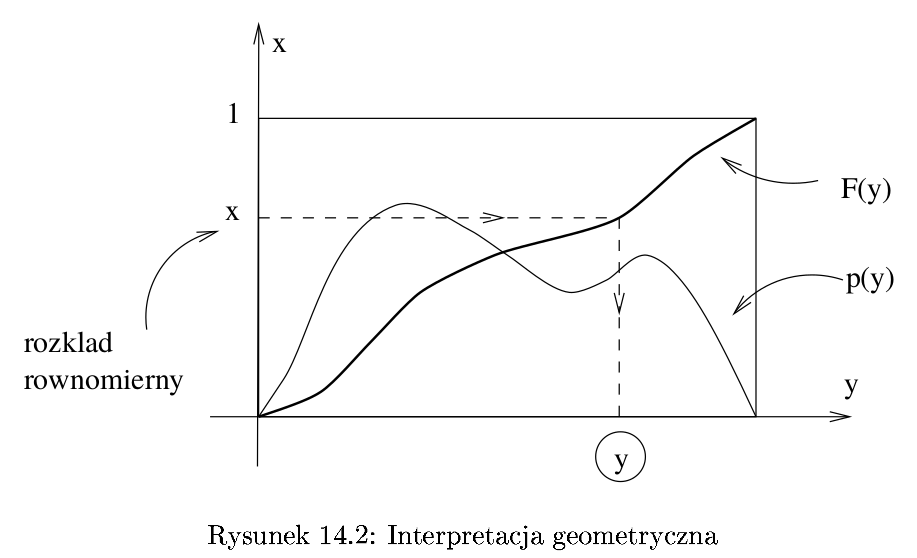
\includegraphics[width=1\linewidth]{img/14/14_6_1_img.png}
\end{frame}
%%%%%%%%%%%%%%
\begin{frame}{Zmienne o rozkładzie normalnym}
	\begin{block}{łączny rozkład prawdopodobieństwa $y$:}
		\[
			p(y_{1},y_{2},\ldots,y_{n})dy_{1}dy_{2} \ldots dy_{n} =
		\]
		\[
			= p(x_{1},x_{2},\ldots,x_{n}) \underbrace{\left|\frac{\partial(x_{1},x_{2},\ldots,x_{n})}{\partial(y_{1},y_{2},\ldots,y_{n})}\right| dy_{1}dy_{2} \ldots dy_{n}}_{dx_{1}dx_{2} \ldots dx_{n}}
		\]
	\end{block}
\end{frame}
%%%%%%%%%%%%%%
\begin{frame}{Metoda Box-Muller (1958)}
	\begin{block}{Metoda Box-Muller (1958) generacji zmiennych losowych o rozkładzie normalnym}
		\[
			p(y)dy = \frac{1}{\sqrt{2\pi}}e^{\frac{y^{2}}{2}}dy \quad, \qquad \text{r. } N(0,1)
		\]
		$x_{1}, x_{2}$ - zm. losowe niezależne, rozkł. równomierny na $(0, 1)$
	\end{block}

	\begin{block}{transformacja:}
		\[
			y_{1} = \sqrt{-2 \ln(x_{1})} \cos(2\pi x_{2})
		\]
		\[
			y_{2} = \sqrt{-2 \ln(x_{1})} \sin(2\pi x_{2})
		\]
	\end{block}
\end{frame}
%%%%%%%%%%%%%%
\begin{frame}{Metoda Box-Muller (1958)}
	\begin{block}{stąd:}
		\[
			x_{1} = \left[- \frac{1}{2} (y_{1}^{2} + y_{2}^{2})\right]
		\]
		\[
			x_{2} = \frac{1}{2\pi} \arctan\frac{y_{1}}{y_{2}}
		\]
	\end{block}
	
	\begin{block}{co daje:}
		\[
			\frac{\partial(x_{1}, x_{2})}{\partial(y_{1}, y_{2})} = \begin{vmatrix}
				\frac{\partial x_{1}}{\partial y_{1}} & \frac{\partial x_{1}}{\partial y_{2}} \\
				\frac{\partial x_{2}}{\partial y_{1}} & \frac{\partial x_{2}}{\partial y_{2}}
			\end{vmatrix} =
			- \left[\frac{1}{\sqrt{2\pi}} e^{-\frac{y_{1}^{2}}{2}}\right] \left[\frac{1}{\sqrt{2\pi}} e^{-\frac{y_{2}^{2}}{2}}\right]
		\]
		$\Rightarrow$ $y_{1} y_{2}$ - każda oddzielnie ma rozkład normalny (2 niezależne!)
	\end{block}
\end{frame}
%%%%%%%%%%%%%%
\begin{frame}{Uproszczenie obliczeń}
	\begin{block}{Zamiast:}
		$x_{1}, x_{2}$ - rozkład równomierny w jednostkowym kwadracie
	\end{block}

	\begin{block}{bierzemy:}
		$v_{1}, v_{2}$ - współrz. punktu w jednostkowym kole:\\
		$v_{1}^{2} + v_{2}^{2} < 1$,\\
		$R = v_{1}^{2} + v_{2}^{2}$ - ma rozkład równomierny - zamiast $x_{1}$\\
		$\angle(v_{1}, v_{2})$ - zamiast $x_{2}$
		\[
			\cos(2\pi x_{2}) = \frac{v_{1}}{\sqrt{R}}; \qquad \sin(2\pi x_{2}) = \frac{v_{2}}{\sqrt{R}}
		\]
		i tak unikamy stosowania funkcji trygonometrycznych
	\end{block}
\end{frame}
%%%%%%%%%%%%%%
\begin{frame}{Uproszczenie obliczeń}
	\begin{block}{}
		\[
			y_{1} = v_{1}\sqrt{\frac{-2 \ln(v_{1}^{2} + v_{2}^{2})}{v_{1}^{2} + v_{2}^{2}}},
		\]
		\[
			y_{2} = y_{1} \cdot \frac{v_{2}}{v_{1}}
		\]
		$y_{1}, y_{2}$ - niezależne, obie o $N(0,1)$
	\end{block}

	\vspace{0.5cm}
	\begin{flushright}
		\textit{Zadanie}
	\end{flushright}

	\vspace{-0.5cm}
	``Numerical Recipes'' rozkłady:
	\begin{itemize}
		\item gamma
		\item Poisona
		\item binominalny (``rejection method'' 7.3)
	\end{itemize}
\end{frame}
	%%%%%%%%%%%%%%%%
	\section{Kryptografia a liczby losowe}
\begin{frame}{Kryptografia a liczby losowe}
	Materiały dostępne w internecie:
	\begin{itemize}
		\item Liczby losowe w kryptografii - \href{http://www.random.mat.sbg.ac.at/}{http://www.random.mat.sbg.ac.at/} (autor: Członek zespołu z University of Salzburg)
	\end{itemize}
\end{frame}
	%%%%%%%%%%%%%%%%

	\begin{frame}
		Źródło:

		N. E. Knuth, ``The Art of Computer Programing vol. II, Addison- Wesley, 1969.

		G.E. Forsythe, M. A. Malcolm, C. R. Mcler, ``Computer Methods for Mathematical Computations 		Prentice Hall, 1977.
	\end{frame}

\end{document}
\grid
